\begin{figure}
  \begin{center}
    \resizebox {.5\columnwidth} {!} {
      \begin{tikzpicture}
        \genealogytree[template=signpost]{
          child{
            g{Agent}
            child{
              g{World Agent}
              child{
                g{Users}
              }
              c{Sources}
            }
            % c[phantom=5em]{aaaaaaa}
            child{
              g{Sky Agent}
              child{
                g{Agent Manager}
                child{
                  g{Agent Manager\\Message Scheduler\\AMMS}
                }
                c{Agent Manager\\Connection Scheduler\\AMCS}
                c{Agent Manager\\Memory Scheduler\\AMME}
              }
            } 
          }
        }
      \end{tikzpicture}
    }
  \end{center}
  \caption{Hierarchy of classes}
  \label{fig:hierarchy}
\end{figure}
\section{Our Model}
We use the SLAPP3 platform for agent simulation: this environment provides agent
based protocol in Python 3.
We implemented a hierarchy of agents to manage the different abilities of
each breed.
\\
The class \textit{Agent} is the common and oldest ancestor,
it has to be so because of SLAPP's structure.\\
Next we have two main classes, defining the main branches,
one for the 'real' agents,\textit{WorldAgent}, and another for
the abstract ones, \textit{SkyAgent}.
The first of the two can represent living creatures or tangible objects;
the second can be thought as an external agent, living outside the world.\\
Of all the classes implemented only five breeds are produced during
the execution of the program.
This structure allows easy changes and possible future implementations
of the code.

\subsection{WorldAgent}
From this branch sprouts two leafs of the tree: the classes \textit{User}
and \textit{Source}.
The common variables passed by \textit{WorldAgent} are
the vector of mind state and the database of news, used both for remember
and as a storage. The common members are trivial.
Specifically talking, the state of mind is a normalized vector of a
specified dimension in the variable \texttt{dim} inside
\textit{commonVar.py}.

\subsubsection{Source}
Sources have a peaked mind state initializated during construction.
The initialization is binary with a number of non zero values from one to three:
after that, noise is added and the vector is normalized.
Each \textit{Source} has a method, \textit{generateNews}, that can produce
a news with a vector of topics inside 'near' the state of the source.
We use near, talking of states, like we talk of geometrical vectors: we will
measure the mind distance with scalar products of these vectors.

\subsubsection{User}
The main class of the program is \textit{User}.
This object contains all the functions to act indipendently in the world.
We will provide a description of the most important ones.
As mentioned before, a user can compute distance, with the homonymous
function, between mind states and between a mind state and a
topic inside news. He can make an opinion of what he sees.
He has a bunch of function to detect who are his neighbours, if they
are sources or users, and if there are only sources around him.
A user can also decide to become active or inactive using internal rules.
He can create or remove an edge between another agent.
Other important actions of users are the way they can diffuse:
\textit{activeDiffusion} and \textit{passiveDiffusion} are the
two functions used to spread news. We will talk about them later.
Finally an agent can choose how and who manage edges with using
\textit{createEdge} and \textit{deleteEdge}.

\subsection{SkyAgent and AgentManager}
\textit{SkyAgent} has an only child: \textit{AgentManager}.
He is responsible of all the logs and the managing of the agent themselves.
Other skyagents can be implemented but we do not need them for now.

\subsubsection{The Schedulers}
There are three leafs out of the \textit{AgentManager's} branch:
\textit{MessageScheduler}, \textit{ConnectionScheduler} and
\textit{MemoryScheduler}. They will be called with their initials,
respectively \textit{AMMS}, \textit{AMCS} and \textit{AMME}.
The purpose of the logs is to provide a post simulation tool to perform
a complete statistical analysis of the model. 
\begin{itemize}
\item [\textit{AMMS}] This scheduler registers all the spreading during the
  execution. It focuses on the news and registers their creation and
  diffusion, also distinguishing the passive and the active diffusion.
\item [\textit{AMCS}] With the connection scheduler we can take note of
  all operations correlated to edges: creation, destruction and weight
  change will be registerd in a log file.
\item [\textit{AMME}] This is unlike the other logs. The call of this log is
  not from an user but from the observer. For every cycle of the program
  this scheduler will print the database of each agent and the activation
  state of anyone.
\end{itemize}

\subsection{Modeling Variables}
It is not easy toi make a decision on modeling human mind. One has to make
a lot of assumprions. For instance, what is important and what is not.
As we have said the agents live in a network. The connections are the
possibility to comunicate and the weight on the edge is like a pregress
trust.

\subsubsection{Mind State}
One choice to model mind is to divide it in topics: the number is arbitrary.
The mind now is a vector where each component is a topic. We chooseto have
non negative values because we model it as anyone can have some interest in
something or not. There is no distinction between having a good or a bad
reputation. One can have or not an opinion.
The initialization of these mind states is initially binary, the vector starts
with only zeros or ones as said for the sources before. Then rumor is added
and the vector is normalized. We chose to have only one peak for users.

\subsubsection{News}
The news is something that someone ca like or dislike. For this reason
it has to be something confrontable with the mind state.
We have built news like  a mind state, near (geometrically speaking)
the source's one. There are other important variables for the news such as
the relevance, which measures the impact of the news in the world, the
date of creation and the source who made it.

\subsection{Execution}
Dynamic is regulated by the scheduled structure of SLAPP. An observer defines
the time of the world while the model itself provides a finer structure of
actions. Furthermore, several actions are scripted and interpreted by
the scheduler.

\subsubsection{Observer}
The observer actions used, included in the file \texttt{observerActions.txt},
are \texttt{modelStep}, \texttt{ask\_all}, \texttt{ask\_one},
\texttt{visualizeNet} and \texttt{clock}.
\begin{itemize}
\item [\texttt{modelStep}] is called with its default implementation
\item [\texttt{ask\_all}] calls the \textit{AMME}
\item [\texttt{ask\_one}] calls the finalization of the program. It
  is used in the last line of the file: the line number has to correspond
  to the final cycle number in order to make the function work.
  To end the execution, log files have to be written, calling
  \texttt{writeLog} which is implemented in each of the \textit{AgentManager's}
  sons. The \texttt{.gml} file of the graph is saved as well as the logs
  in a folder created ah hoc: \texttt{logs}.
  If the execution interrupts or, for some reason, \texttt{ask\_one} is not
  called properly, the files would be saved as well in a temporary folder,
  \texttt{temp}, and the logs would be saved until the last
  automatic save (every 1000 lines of log).
\item [\texttt{visualizeNet}] calls the net visualizzation. The function called
  is \texttt{drawGraph} contained in the file \texttt{graph.py}.
  From there is possible to draw the net, to save the file or both.
\item [\texttt{clock}] increments the world time 
\end{itemize}

\begin{figure}[htpb]
  \centering
  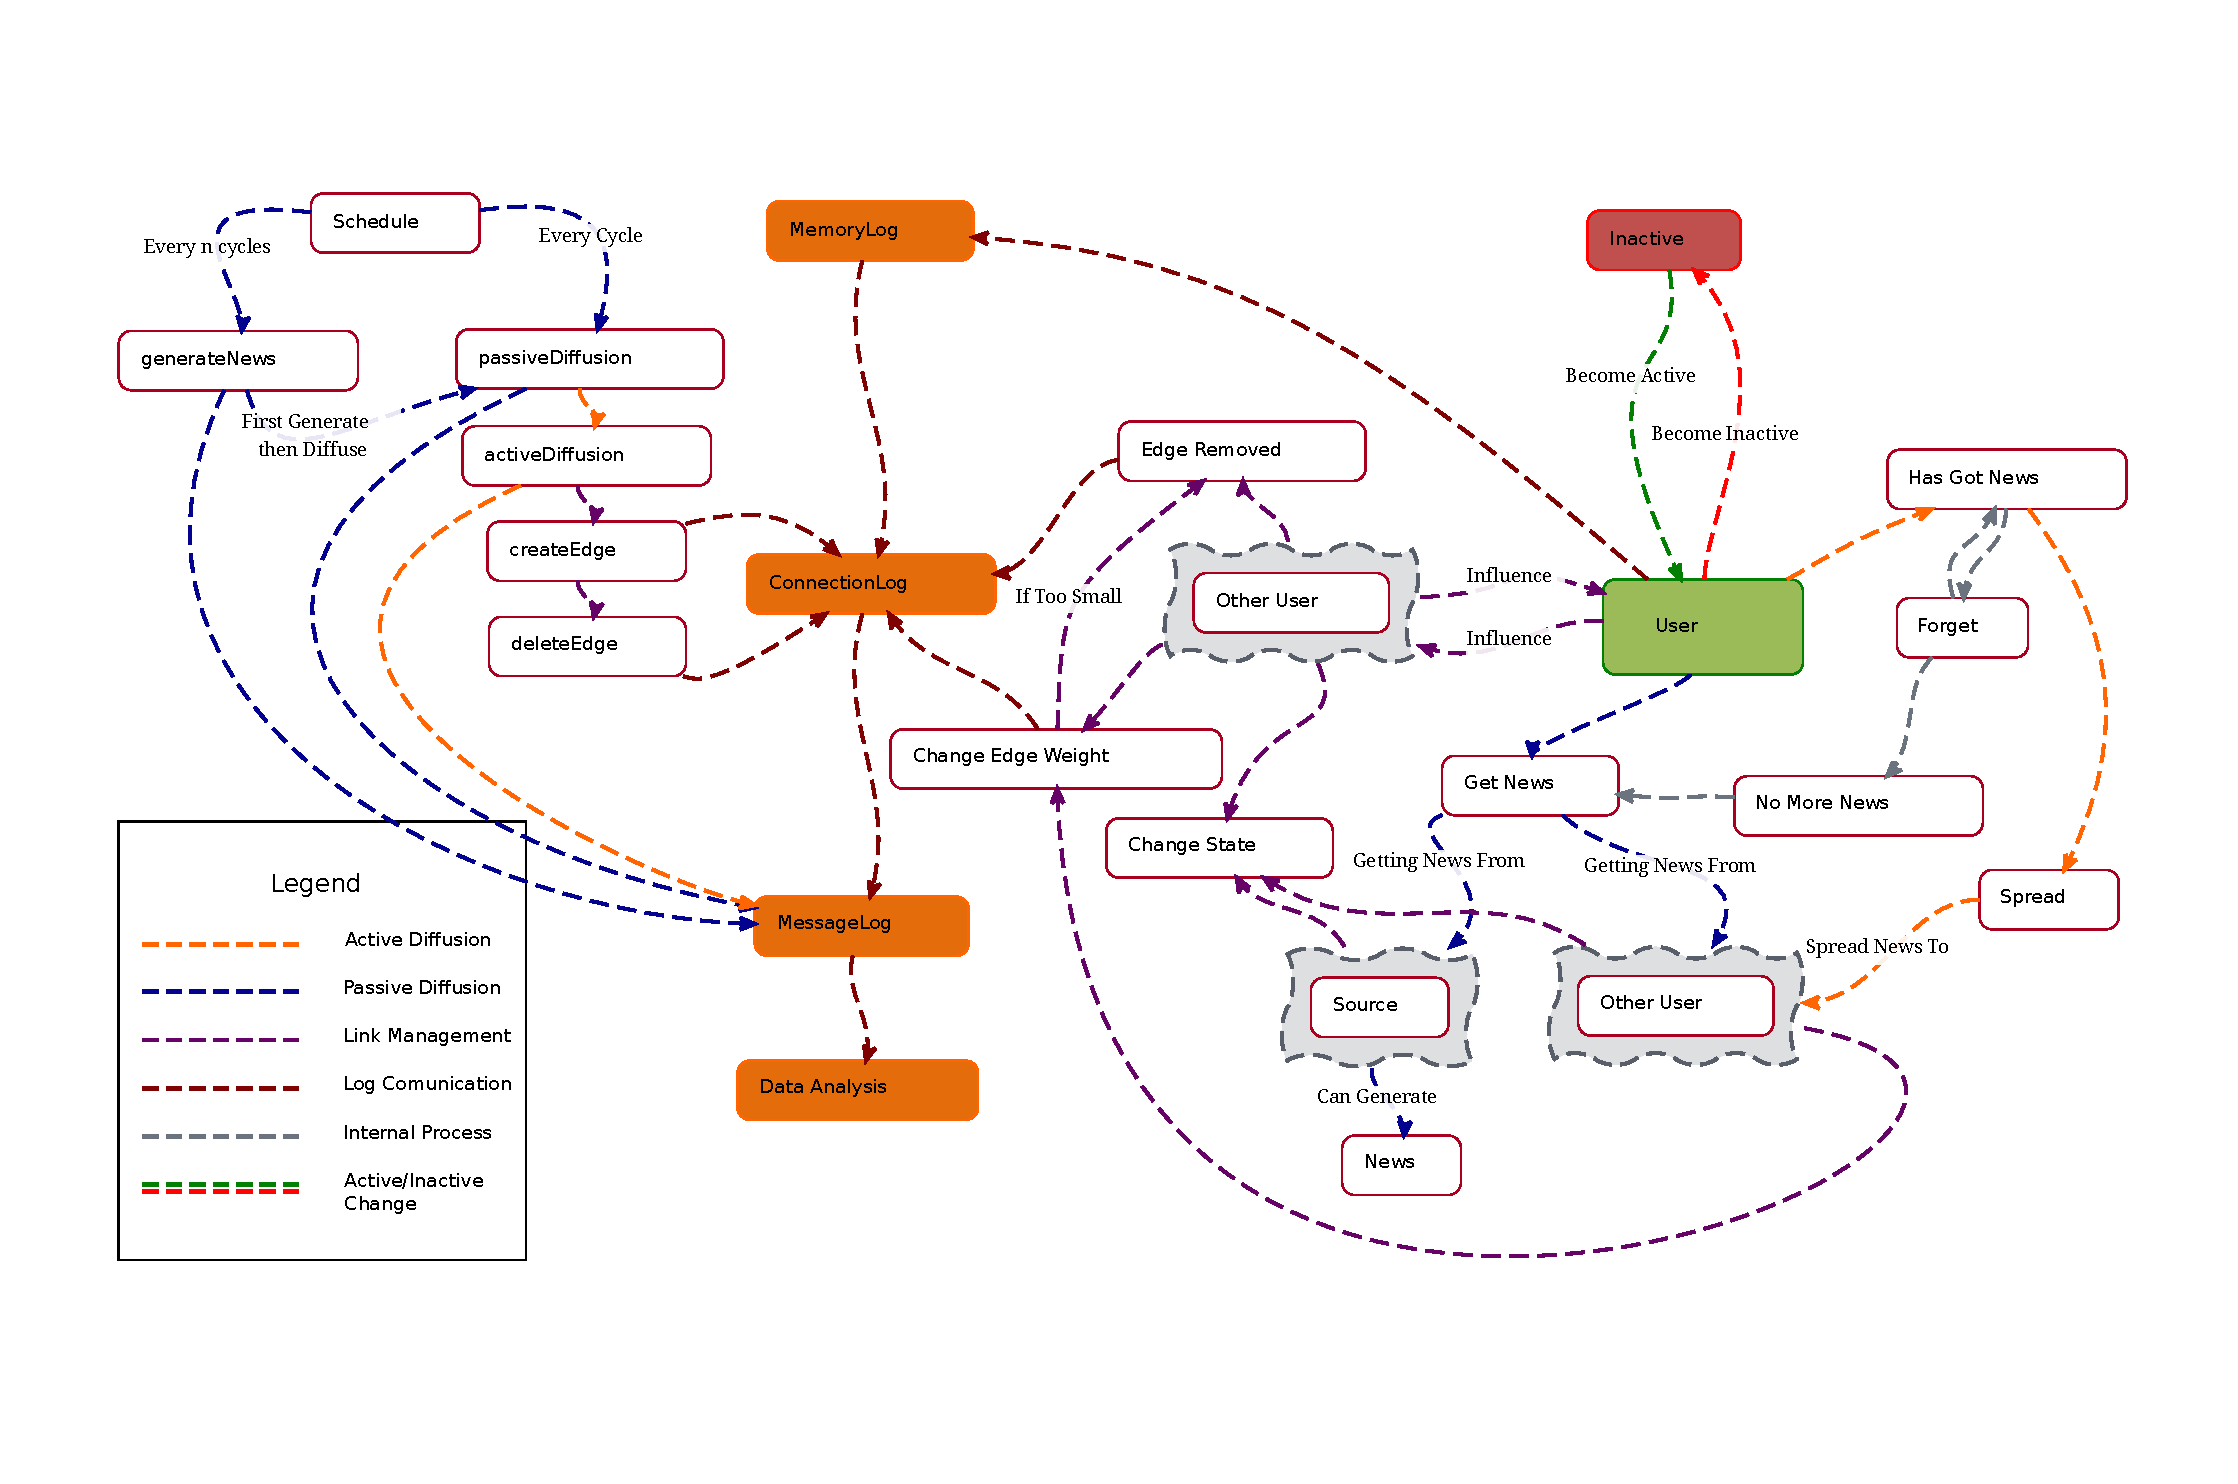
\includegraphics[trim={2cm 3cm 1.5cm 2cm}, clip,width=\columnwidth]{img/pdf/mindMap.pdf}
  \caption{Mind map of the model}
  \label{fig:mindmap}
\end{figure}

\subsubsection{Model and Schedule}
The file \texttt{modelActions.txt} calls for every cycle the script with
\texttt{read\_script}.
The \texttt{reset} and \texttt{move} functions are not implemented
but still called as placeholders.
The file \texttt{schedule.xls} makes five calls:
\begin{itemize}
\item [timestep 1] during the first cycle the program generates news
  contained in the sources;
\item [timesteps 2 - 10000] after news generation and for all
  the execution, users make passive and active diffusion;
\item [timesteps 10 - 10000] after some time of diffusion the agents start
  to modify the net structure, adding and removing edges with a probability
  of 0.03.
\end{itemize}

\subsection{Overview on simulation: technical difficulties}
Focus on a complete cycle of simulation, dealing with some
practical details, while the overview of the main process is given to be
clear to the reader. The figure~\ref{fig:mindmap} explains the main program
workflow during a generic simulation.
From left to right: the schedule runs the main blocks, then the logs start
the acquisition of data, finally we see the actions of a generic agent
during one time step.

\subsubsection{The problem of 'log calling' and 'memory unload'}
The breed order creation is log first, then users and finally sources.
We will discuss how and where to call a log during the execution of the program.
As we previously said, logs are agents themselves, not external functions
or tools. The problem is how to call a log at runtime; this is solved
only when a single instance of every \textit{AgentManager's} son is
created. Each scheduler, automatically builds himself, during
initialization, inside the commonVar.py file. It is obvious how this trick
would not work for more than one log for breed.
The agent nature of the log is not a bad thing at all. All the logs are
able to manage the memory autonomously: they full the memory of the machine
until a limit value of lines and then autosave, appending all the work done
in a temporary file. This provides a limited number of access to the disk and
a reasonable amount of memory used during the simulation.

\subsubsection{How to create a graph of agents:
  'further implementation issue'}
The class \textit{WorldAgent} creates the graph during the agent
initialziation. The trick used is clever but can produce some
problems in further implementations. The first agent creates the graph
if he is the first called and if the timestep is the initial; all the
agents append themselves at initialization and the last one creates the edges
randomly. This is a problem if we want to implement a feature for adding nodes.
What we want to avoid is the re-initialization of edges at every new
\textit{WorldAgent} initialization. If the number of agents does not change the
simulation works properly.

\subsubsection{Determinism and Random}
The decision taken by agents are half deterministic and half random.
Let's take for instance the action \texttt{addEdge}.
An agent of the breed user can decide to add a node choosig from the
other agents in the net.
He choose between a user chosen randomly in the net and one beween
his second nearest neighbours.
The way he choose is making the distance between his mind state and the
possible future linked agent's mind state. To add a bit of randomness
in this deterministic choice the agent adds all the second nearest
neighbours in a list, sorted by distance from his state and counted
with their multiplicity. Then he chooses randomly from the first ten
elements of the sorted list. In this way we cam model rules for the
actions but make the behaviour unpredictable adding random.

\subsection{What can this model do?}
This can be used for simulate the spread of one or more news generated
by sources at any cycle of time. The news can also be added or regenerated
every time. It can run for an arbitrary long mind state of agents,
for an arbitrary memory length.
It is written using dictionaries so provides a very small time to process data.
Other mathematical operations are performed including numpy.
Furthrtmore it can run very long symulations considering the possibility
of deciding not to save graphs and only producing logs for post simulation
analysis.
